\addcontentsline{toc}{section}{\textbf{CAPÍTULO V}}
\addcontentsline{toc}{section}{\textbf{ADMINISTRACIÓN DEL PROYECTO}}

\subsection{Cronograma de actividades}

El proyecto de investigación se desarrollará durante el año académico
2026, organizado en seis fases secuenciales, con una duración total de
seis meses. Las Tablas \ref{tab:cronograma1} y \ref{tab:cronograma2}
presentan la distribución temporal de las actividades por fase, desde
la planificación y revisión bibliográfica hasta la evaluación final del
sistema y el análisis estadístico de los resultados.

%====================================================
% EL ENTORNO LANDSCAPE DEBE EMPEZAR RECIÉN AQUÍ
%====================================================

\begin{landscape}
\begin{table}[htbp]
\centering
\small

\caption{Cronograma de actividades -- Fases I a III (Julio -- Diciembre 2026)}
\label{tab:cronograma1}

\renewcommand{\arraystretch}{1.55}
\setlength{\tabcolsep}{4.2pt}

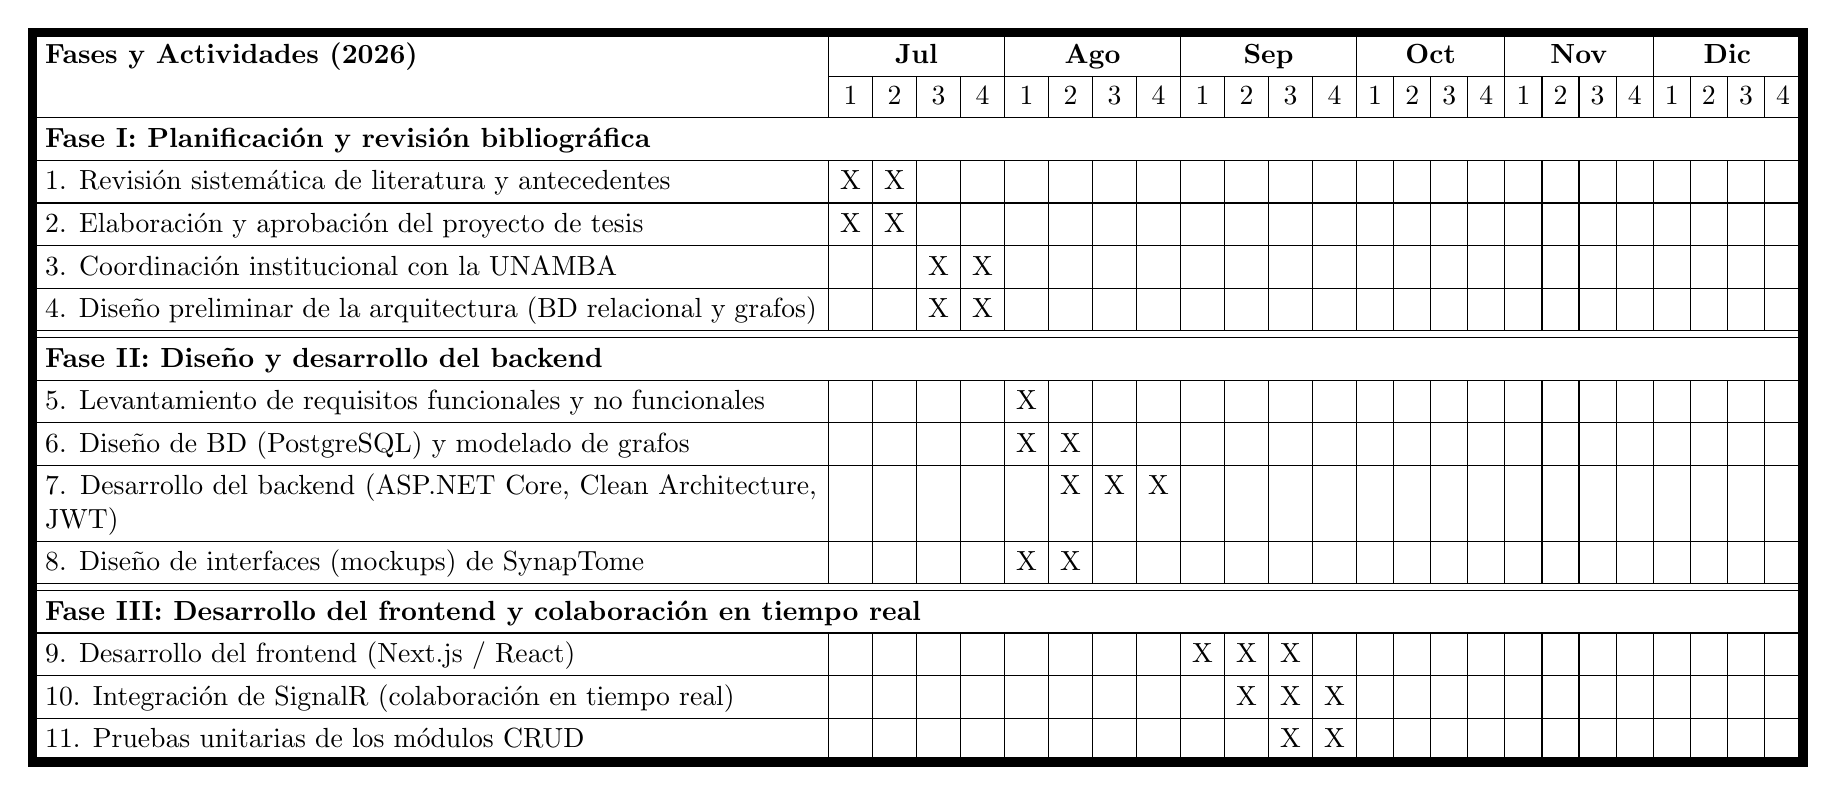
\begin{tikzpicture}
\node[inner sep=0pt] (tabla) {
\begin{tabular}{|p{9.8cm}|c|c|c|c|c|c|c|c|c|c|c|c|c|c|c|c|c|c|c|c|c|c|c|c|}
\hline
\textbf{Fases y Actividades (2026)}
& \multicolumn{4}{c|}{\textbf{Jul}} & \multicolumn{4}{c|}{\textbf{Ago}} & \multicolumn{4}{c|}{\textbf{Sep}} & \multicolumn{4}{c|}{\textbf{Oct}} & \multicolumn{4}{c|}{\textbf{Nov}} & \multicolumn{4}{c|}{\textbf{Dic}} \\
\cline{2-25}
 & 1&2&3&4 & 1&2&3&4 & 1&2&3&4 & 1&2&3&4 & 1&2&3&4 & 1&2&3&4 \\
\hline
\thickhline

\multicolumn{25}{|l|}{\textbf{Fase I: Planificación y revisión bibliográfica}} \\
\hline
%                                    J1 J2 J3 J4  A1 A2 A3 A4  S1 S2 S3 S4  O1 O2 O3 O4  N1 N2 N3 N4  D1 D2 D3 D4
1. Revisión sistemática de literatura y antecedentes
& X & X &  &  &  &  &  &  &  &  &  &  &  &  &  &  &  &  &  &  &  &  &  &  \\
\hline
2. Elaboración y aprobación del proyecto de tesis
& X & X &  &  &  &  &  &  &  &  &  &  &  &  &  &  &  &  &  &  &  &  &  &  \\
\hline
3. Coordinación institucional con la UNAMBA
&  &  & X & X &  &  &  &  &  &  &  &  &  &  &  &  &  &  &  &  &  &  &  &  \\
\hline
4. Diseño preliminar de la arquitectura (BD relacional y grafos)
&  &  & X & X &  &  &  &  &  &  &  &  &  &  &  &  &  &  &  &  &  &  &  &  \\
\hline
\hline

\multicolumn{25}{|l|}{\textbf{Fase II: Diseño y desarrollo del backend}} \\
\hline
5. Levantamiento de requisitos funcionales y no funcionales
&  &  &  &  & X &  &  &  &  &  &  &  &  &  &  &  &  &  &  &  &  &  &  &  \\
\hline
6. Diseño de BD (PostgreSQL) y modelado de grafos
&  &  &  &  & X & X &  &  &  &  &  &  &  &  &  &  &  &  &  &  &  &  &  &  \\
\hline
7. Desarrollo del backend (ASP.NET Core, Clean Architecture, JWT)
&  &  &  &  &  & X & X & X &  &  &  &  &  &  &  &  &  &  &  &  &  &  &  &  \\
\hline
8. Diseño de interfaces (mockups) de SynapTome
&  &  &  &  & X & X &  &  &  &  &  &  &  &  &  &  &  &  &  &  &  &  &  &  \\
\hline
\hline

\multicolumn{25}{|l|}{\textbf{Fase III: Desarrollo del frontend y colaboración en tiempo real}} \\
\hline
9. Desarrollo del frontend (Next.js / React)
&  &  &  &  &  &  &  &  & X & X & X &  &  &  &  &  &  &  &  &  &  &  &  &  \\
\hline
10. Integración de SignalR (colaboración en tiempo real)
&  &  &  &  &  &  &  &  &  & X & X & X &  &  &  &  &  &  &  &  &  &  &  &  \\
\hline
11. Pruebas unitarias de los módulos CRUD
&  &  &  &  &  &  &  &  &  &  & X & X &  &  &  &  &  &  &  &  &  &  &  &  \\
\hline
\end{tabular}
};

%====================================================
% ENCUADRE DE BORDE GRUESO UNIVERSITARIO (3.5pt)
%====================================================
\draw[line width=3.5pt] (tabla.north west) rectangle (tabla.south east);
\end{tikzpicture}
\end{table}
\end{landscape}


\begin{landscape}
\begin{table}[htbp]
\centering
\small

\caption{Cronograma de actividades -- Fases IV a VI (Julio -- Diciembre 2026)}
\label{tab:cronograma2}

\renewcommand{\arraystretch}{1.55}
\setlength{\tabcolsep}{4.2pt}

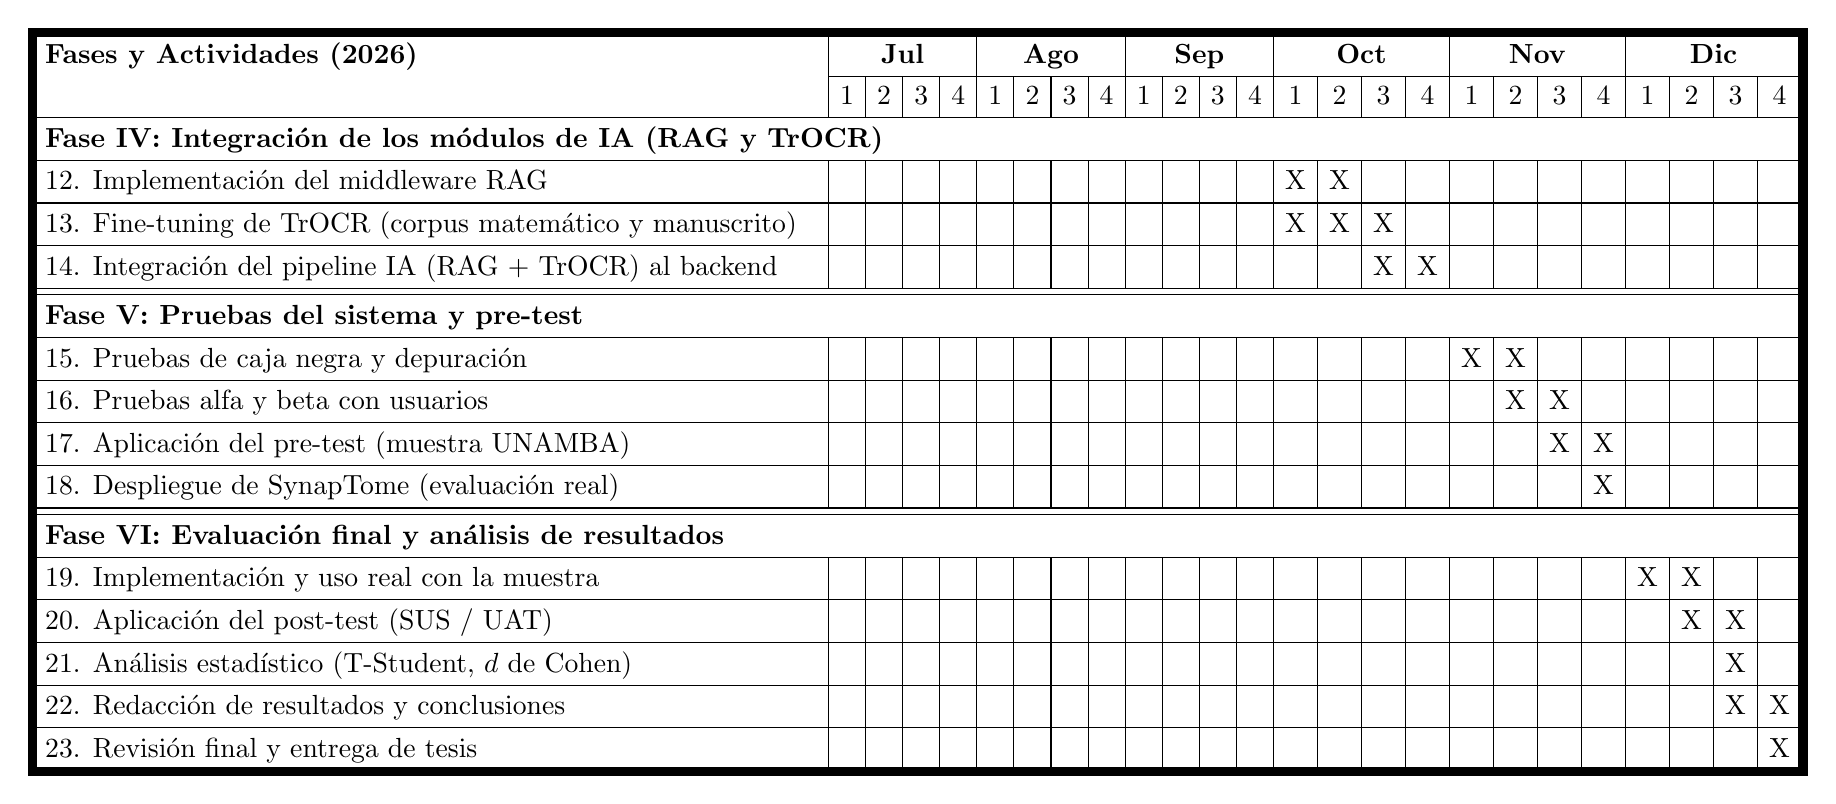
\begin{tikzpicture}
\node[inner sep=0pt] (tabla2) {
\begin{tabular}{|p{9.8cm}|c|c|c|c|c|c|c|c|c|c|c|c|c|c|c|c|c|c|c|c|c|c|c|c|}
\hline
\textbf{Fases y Actividades (2026)}
& \multicolumn{4}{c|}{\textbf{Jul}} & \multicolumn{4}{c|}{\textbf{Ago}} & \multicolumn{4}{c|}{\textbf{Sep}} & \multicolumn{4}{c|}{\textbf{Oct}} & \multicolumn{4}{c|}{\textbf{Nov}} & \multicolumn{4}{c|}{\textbf{Dic}} \\
\cline{2-25}
 & 1&2&3&4 & 1&2&3&4 & 1&2&3&4 & 1&2&3&4 & 1&2&3&4 & 1&2&3&4 \\
\hline
\thickhline

\multicolumn{25}{|l|}{\textbf{Fase IV: Integración de los módulos de IA (RAG y TrOCR)}} \\
\hline
%                              J1 J2 J3 J4  A1 A2 A3 A4  S1 S2 S3 S4  O1 O2 O3 O4  N1 N2 N3 N4  D1 D2 D3 D4
12. Implementación del middleware RAG
&  &  &  &  &  &  &  &  &  &  &  &  & X & X &  &  &  &  &  &  &  &  &  &  \\
\hline
13. Fine-tuning de TrOCR (corpus matemático y manuscrito)
&  &  &  &  &  &  &  &  &  &  &  &  & X & X & X &  &  &  &  &  &  &  &  &  \\
\hline
14. Integración del pipeline IA (RAG + TrOCR) al backend
&  &  &  &  &  &  &  &  &  &  &  &  &  &  & X & X &  &  &  &  &  &  &  &  \\
\hline
\hline

\multicolumn{25}{|l|}{\textbf{Fase V: Pruebas del sistema y pre-test}} \\
\hline
15. Pruebas de caja negra y depuración
&  &  &  &  &  &  &  &  &  &  &  &  &  &  &  &  & X & X &  &  &  &  &  &  \\
\hline
16. Pruebas alfa y beta con usuarios
&  &  &  &  &  &  &  &  &  &  &  &  &  &  &  &  &  & X & X &  &  &  &  &  \\
\hline
17. Aplicación del pre-test (muestra UNAMBA)
&  &  &  &  &  &  &  &  &  &  &  &  &  &  &  &  &  &  & X & X &  &  &  &  \\
\hline
18. Despliegue de SynapTome (evaluación real)
&  &  &  &  &  &  &  &  &  &  &  &  &  &  &  &  &  &  &  & X &  &  &  &  \\
\hline
\hline

\multicolumn{25}{|l|}{\textbf{Fase VI: Evaluación final y análisis de resultados}} \\
\hline
19. Implementación y uso real con la muestra
&  &  &  &  &  &  &  &  &  &  &  &  &  &  &  &  &  &  &  &  & X & X &  &  \\
\hline
20. Aplicación del post-test (SUS / UAT)
&  &  &  &  &  &  &  &  &  &  &  &  &  &  &  &  &  &  &  &  &  & X & X &  \\
\hline
21. Análisis estadístico (T-Student, $d$ de Cohen)
&  &  &  &  &  &  &  &  &  &  &  &  &  &  &  &  &  &  &  &  &  &  & X &  \\
\hline
22. Redacción de resultados y conclusiones
&  &  &  &  &  &  &  &  &  &  &  &  &  &  &  &  &  &  &  &  &  &  & X & X \\
\hline
23. Revisión final y entrega de tesis
&  &  &  &  &  &  &  &  &  &  &  &  &  &  &  &  &  &  &  &  &  &  &  & X \\
\hline
\end{tabular}
};

%====================================================
% ENCUADRE DE BORDE GRUESO UNIVERSITARIO (3.5pt)
%====================================================
\draw[line width=3.5pt] (tabla2.north west) rectangle (tabla2.south east);
\end{tikzpicture}
\end{table}
\end{landscape}


\subsection{Presupuesto}

La Tabla \ref{tab:presupuesto} presenta el presupuesto estimado para
el desarrollo del proyecto de investigación, organizado por categorías
de gasto. Las principales herramientas de software (Visual Studio,
.NET SDK, Next.js y Jamovi) se utilizarán bajo licencias gratuitas u
\textit{open source}, mientras que los principales costos corresponden
al consumo de APIs de modelos de lenguaje, al hosting del sistema y a
la aplicación de instrumentos a la muestra de estudiantes.

\begin{table}[H]
\centering
\small
\caption{Presupuesto estimado del proyecto de investigación}
\label{tab:presupuesto}

\renewcommand{\arraystretch}{1.25}
\setlength{\tabcolsep}{4pt}

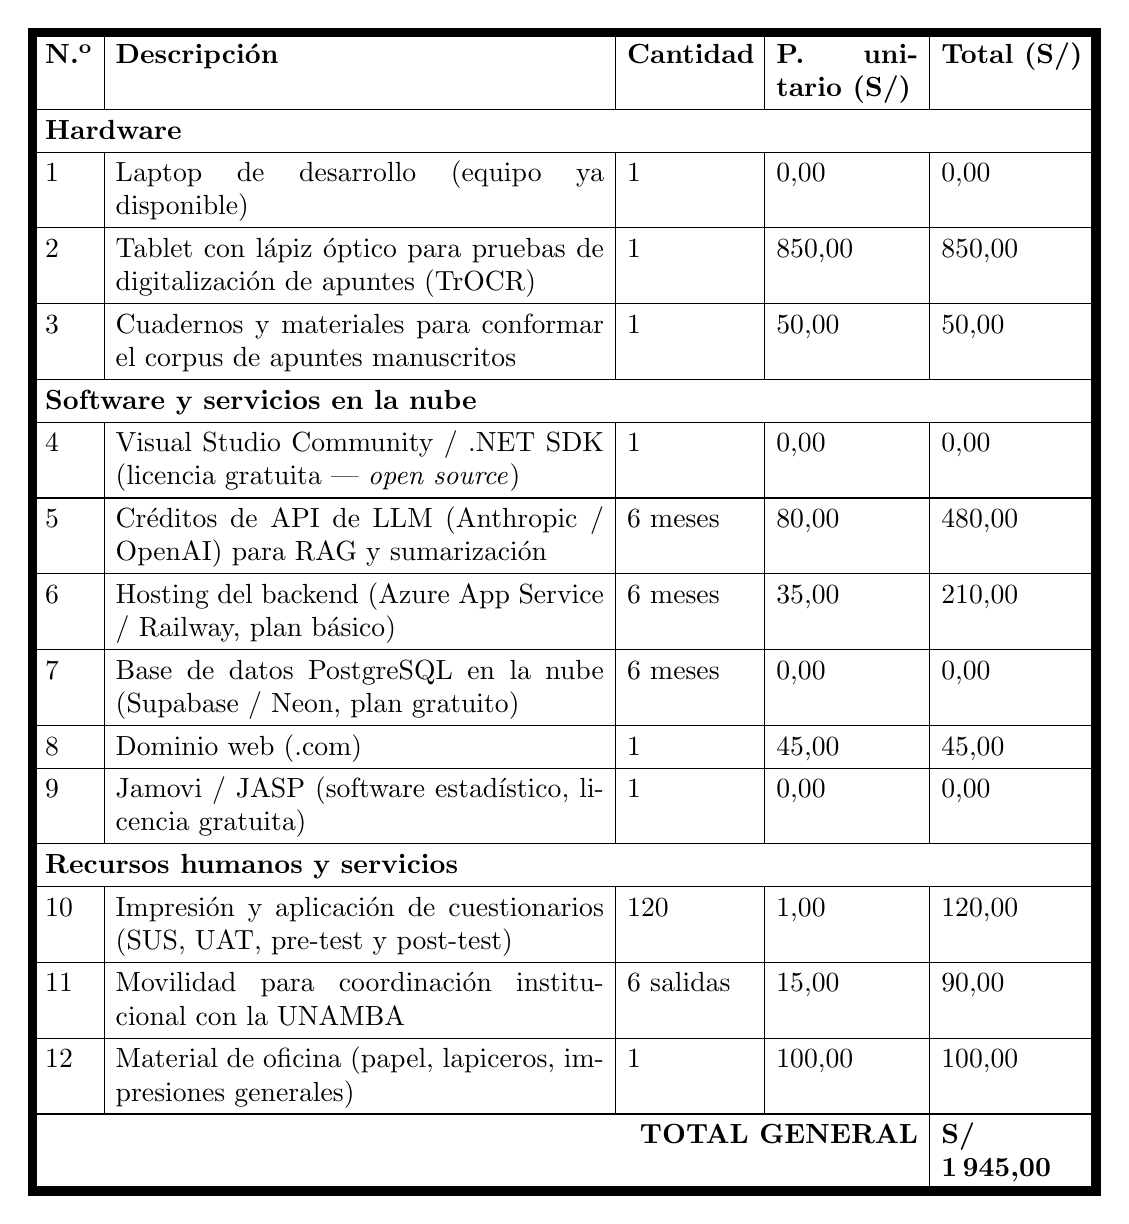
\begin{tikzpicture}
\node[inner sep=0pt] (table) {
\begin{tabular}{|p{0.6cm}|p{6.2cm}|p{1.6cm}|p{1.8cm}|p{1.8cm}|}

\hline
\textbf{N.\textsuperscript{o}} &
\textbf{Descripción} &
\textbf{Cantidad} &
\textbf{P. unitario (S/)} &
\textbf{Total (S/)} \\
\hline
\thickhline

\multicolumn{5}{|l|}{\textbf{Hardware}} \\
\hline
1 & Laptop de desarrollo (equipo ya disponible) &
1 & 0,00 & 0,00 \\
\hline
2 & Tablet con lápiz óptico para pruebas de digitalización de apuntes (TrOCR) &
1 & 850,00 & 850,00 \\
\hline
3 & Cuadernos y materiales para conformar el corpus de apuntes manuscritos &
1 & 50,00 & 50,00 \\
\hline

\multicolumn{5}{|l|}{\textbf{Software y servicios en la nube}} \\
\hline
4 & Visual Studio Community / .NET SDK (licencia gratuita --- \textit{open source}) &
1 & 0,00 & 0,00 \\
\hline
5 & Créditos de API de LLM (Anthropic / OpenAI) para RAG y sumarización &
6 meses & 80,00 & 480,00 \\
\hline
6 & Hosting del backend (Azure App Service / Railway, plan básico) &
6 meses & 35,00 & 210,00 \\
\hline
7 & Base de datos PostgreSQL en la nube (Supabase / Neon, plan gratuito) &
6 meses & 0,00 & 0,00 \\
\hline
8 & Dominio web (.com) &
1 & 45,00 & 45,00 \\
\hline
9 & Jamovi / JASP (software estadístico, licencia gratuita) &
1 & 0,00 & 0,00 \\
\hline

\multicolumn{5}{|l|}{\textbf{Recursos humanos y servicios}} \\
\hline
10 & Impresión y aplicación de cuestionarios (SUS, UAT, pre-test y post-test) &
120 & 1,00 & 120,00 \\
\hline
11 & Movilidad para coordinación institucional con la UNAMBA &
6 salidas & 15,00 & 90,00 \\
\hline
12 & Material de oficina (papel, lapiceros, impresiones generales) &
1 & 100,00 & 100,00 \\

\hline
\multicolumn{4}{|r|}{\textbf{TOTAL GENERAL}} &
\textbf{S/ 1\,945,00} \\
\hline

\end{tabular}
};

\draw[line width=3.5pt]
(table.north west) rectangle (table.south east);
\end{tikzpicture}

\end{table}


\subsection{Fuente de financiamiento}

El presente proyecto de investigación será financiado íntegramente
con recursos propios del investigador. La mayor parte de las
herramientas de software utilizadas (Visual Studio, .NET SDK, Next.js,
React y Jamovi) son de acceso gratuito o de código abierto, mientras
que los servicios en la nube (créditos de API de LLM, hosting y base
de datos) se mantienen dentro de planes básicos o niveles gratuitos,
lo que reduce significativamente los costos del proyecto.